\chapter{Задание}

Разработать графический интерфейс, который позволяет по заданной
матрице интенсивностей перехода состояний определить время пребывания
системы в каждом состоянии в установившемся режиме работы системы.
Для каждого состояния также требуется рассчитать предельную вероятность.
Количество состояний не более десяти.

\chapter{Теоретическая часть}

\section{Марковский процесс}

Случайный процесс называется марковским процессом, если для каждого момента времени $t$ вероятность любого состояния системы в будущем зависит только от ее состояния в настоящем и не зависит от того, как система пришла в это состояние.

\section{Предельная вероятность}

Для определения предельной вероятности необходимо решить систему уравнений Колмагорва, в которой все производные приравниваются к нулю, а одно из уравнений заменяется на условие нормировки:

\begin{equation}
    \begin{aligned}
        \sum_{j = 1}^{n} p_{j}(t) = 1.
    \end{aligned}
\end{equation}

\section{Точки стабилизации состояния системы}

Для определения точек стабилизации состояния системы нужно определить вероятности нахождения в определённых состояниях с некоторым малым шагом $\Delta t$. В тот момент, когда разница между вычисленной на данном шаге вероятностью и предельной вероятности будет достаточно мала (< $EPS$), то точка стабилизации считается найденной.


\chapter{Результаты работы}

\section{Листинги программы}

В листинге \ref{lst:markovChains} представлен класс $MarkovChains$, отвечающий за определение времени пребывания системы в каждом состоянии в установившемся режиме работы системы и за рассчет предельных вероятностей.

\begin{lstlisting}[label=lst:markovChains, caption=class MarkovChains]
import numpy as np
from scipy.integrate import odeint
import matplotlib.pyplot as plt

EPS = 1e-3
class MarkovChains():
    matrix: list
    matrixSize: int

    initProbs: list
    dt: float

    def __init__(self, matrix: int, matrixSize: int, dt: float):
        self.matrix = matrix
        self.matrixSize = matrixSize
        self.initProbs = self.createInitProbabilities(matrixSize)
        self.dt = dt

    def createInitProbabilities(self, arraySize):
        return [1 if i == 0 else 0 for i in range(arraySize)]
  
    def getProbabilities(self):
        freeMembers = [0 for _ in range(self.matrixSize - 1)]
        freeMembers.append(1)

        matrixСoeffs = [
            [
                -sum(self.matrix[i]) + self.matrix[i][j] if j == i else self.matrix[j][i] 
                for j in range(self.matrixSize)
            ]
            for i in range(self.matrixSize - 1)
        ]
        matrixСoeffs.append([1 for _ in range(self.matrixSize)])

        # Стабильное состояние
        probsSteady = np.linalg.solve(matrixСoeffs, freeMembers)

        return probsSteady

    def solveOde(self, initProbs: list, _, matrixСoeffs: list):
        dydt = [0 for _ in range(self.matrixSize)]
        
        for i in range(self.matrixSize):
            dydt[i] = sum(initProbs[j] * matrixСoeffs[i][j] for j in range(self.matrixSize))

        return dydt

    def getTimes(self, probsSteady: list, buildGraph: bool):
        matrixСoeffs = [
            [
                -sum(self.matrix[i]) + self.matrix[i][j] if j == i else self.matrix[j][i] 
                for j in range(self.matrixSize)
            ]
            for i in range(self.matrixSize)
        ]
        times = np.arange(0, 20, self.dt)
    
        resOde = odeint(self.solveOde, self.initProbs, times, args=(matrixСoeffs,))
        resOde = np.transpose(resOde)

        timesSteady = list()

        for i in range(self.matrixSize):
            if buildGraph:
                plt.plot(times, resOde[i], label = "p{}".format(i))

            for j in range(len(resOde[i]) - 1, -1, -1):
                if abs(probsSteady[i] - resOde[i][j]) > EPS:
                    # Времена достижения стабильного состояния
                    timesSteady.append(times[j])
                    break
        if buildGraph:
            plt.legend()
            plt.grid()
            plt.show()

        return timesSteady

    def solve(self, buildGraph: bool):
        probsSteady = self.getProbabilities()
        timesSteady = self.getTimes(probsSteady, buildGraph)

        return [probsSteady, timesSteady]
\end{lstlisting}

\clearpage

\section{Демонстрация работы программы}

На рисунках \ref{img:matrix3} - \ref{img:graph10} представлены примеры работы программы.

\begin{figure}[h]
    \centering
    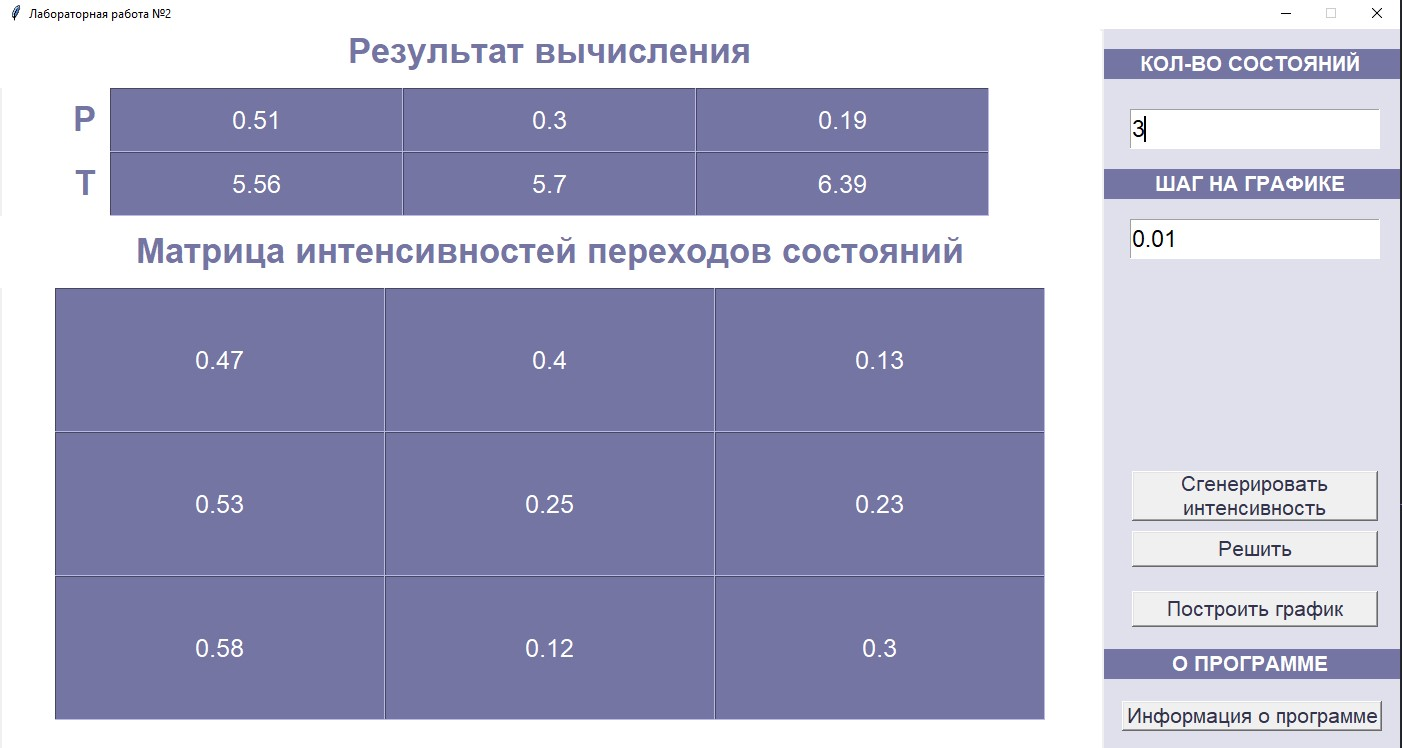
\includegraphics[scale = 0.4]{img/3.jpg}
    \caption{Система из 3 состояний}
    \label{img:matrix3}
\end{figure}

\begin{figure}[h]
    \centering
    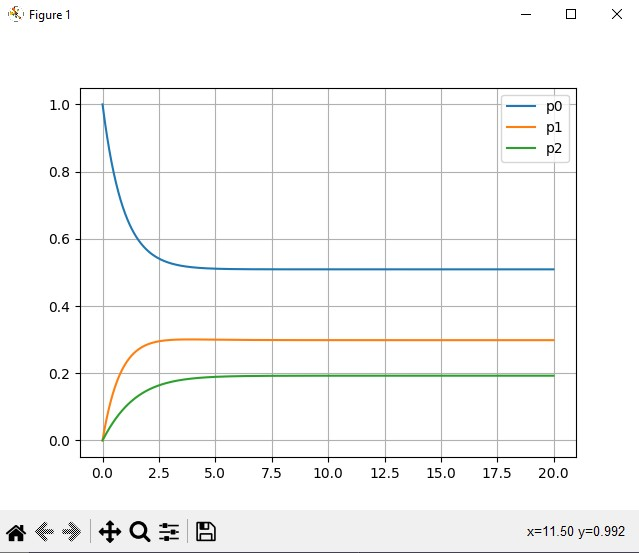
\includegraphics[scale = 0.6]{img/3g.jpg}
    \caption{График вероятности от времени для системы из 3 состояний}
    \label{img:graph3}
\end{figure}

\begin{figure}[h]
    \centering
    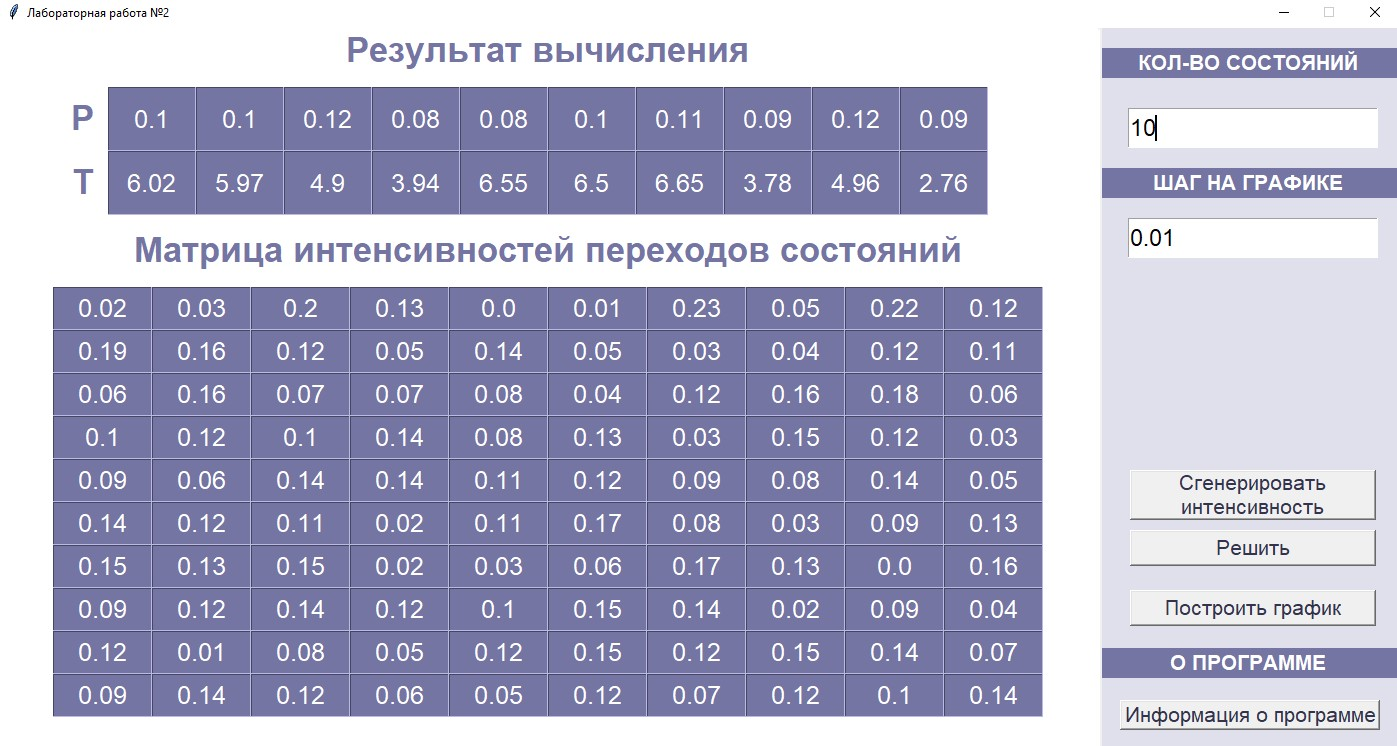
\includegraphics[scale = 0.4]{img/10.jpg}
    \caption{Система из 10 состояний}
    \label{img:matrix10}
\end{figure}

\begin{figure}[h]
    \centering
    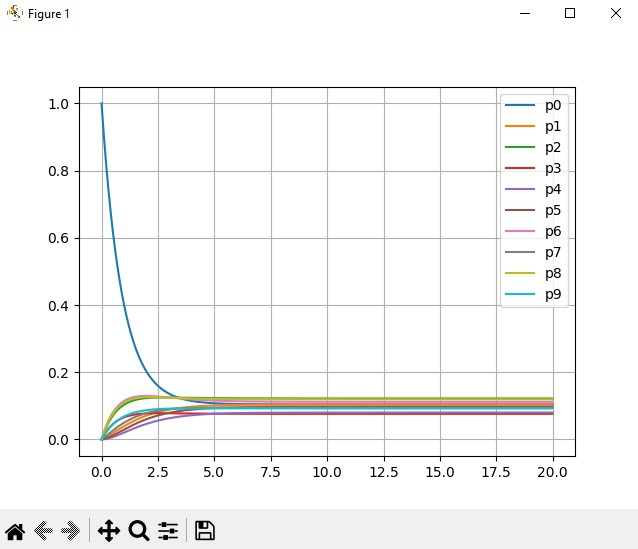
\includegraphics[scale = 0.6]{img/10g.jpg}
    \caption{График вероятности от времени для системы из 10 состояний}
    \label{img:graph10}
\end{figure}